\documentclass[letter,12 pt,titlepage]{article}
 
\usepackage[utf8]{inputenc}
\usepackage[spanish]{babel}
\usepackage[T1]{fontenc}
\usepackage{lmodern}
\usepackage{amssymb}
\usepackage{parskip}
\usepackage{xcolor}
\usepackage{multicol}
\usepackage{anysize}
\usepackage{enumerate}
\usepackage{url}
\usepackage{pdfpages}
\usepackage[hidelinks]{hyperref}
\usepackage{chngcntr}
\counterwithout{footnote}{section}
\usepackage{float}

%izq der arr ab
\marginsize{2.5 cm}{2.5 cm}{1 cm}{1 cm} 

\begin{document}
    \begin{titlepage}
        \centering
        
\includegraphics[width=0.15\textwidth]{img/escudo_fi_color.png}\par\vspace{1cm}
        {\scshape\LARGE Facultad de Ingeniería \par}
        \vspace{1cm}
        {\scshape\Large Estructura y Programación de Computadoras
        \par}
        \vspace{1cm}
        {\scshape\Large Grupo 2
        \par}
        \vspace{1.5cm}
        {\huge\bfseries Proyecto Nº1\par}
        \vspace{2cm}
        {\Large 
            Martínez Baeza José Alfonso
        \par}
        \vfill
        {\large 22 de abril de 2020\par}
    \end{titlepage}
    \newpage
    \tableofcontents
    \newpage

    \section{Introducción}

    \subsection{Descripción del problema}

        Se requiere elaborar un programa que realice operaciones básicas entre dos números ingreseados por el usuario y que muestre los resultados en pantalla.

    \subsection{Planteamiento del problema}

        Desarrollar un programa en lenguaje ensamblador para arquitectura Intel x86 que solicite ingresar 2 números desde el teclado, y que calcule:
        
        \begin{center}
            \begin{minipage}{0.95\linewidth}
                \begin{itemize}
                    \item La suma de ambos números.
                    \item La resta del primer número menos el segundo.
                    \item La multiplicación de ambos números.
                    \item El cociente de la división del primer número entre el segundo.
                    \item El residuo de la división del primer número entre el segundo.
                \end{itemize}
            \end{minipage}
        \end{center}

        \textbf{Consideraciones:}
        \begin{center}
            \begin{minipage}{0.95\linewidth}
                \begin{itemize}
                    \item Los números deben estar en sistema decimal (dígitos de 0-9).
                    \item Los números deberán ser enteros sin signo.
                    \item Cada número introducido por el usuario puede ser de hasta 4 dígitos. El programa debe restringir que el usuario introduzca más números.
                    \item Al ingresar los números, no deberá aceptar caracteres que no sean numéricos.
                \end{itemize}
            \end{minipage}
        \end{center}

    \section{Desarrollo}

    Para la realización de este proyecto nos apoyaremos del uso de macros y procedimientos dentro del lenguaje ensamblador para poder reducir el número de líneas de código, también se hará uso de saltos condicionales, variables auxiliares, etc.

    \subsection{Macros}

    Se programaron dos macros en este proyecto: \textit{clear} y \textit{delete} para limpiar la pantalla y eliminar un caracter respectivamente.

    \subsubsection{Clear}
    Esta macro se encarga de limpiar la pantalla cada que el usuario inicia o finaliza la ejecución del programa.
    Hace uso de la interrupción $10h$ \footnote{\url{http://ict.udlap.mx/people/oleg/docencia/Assembler/asm_interrup_10.html}}, junto con el valor $00h$ selecciona y activa el modo de vídeo especificado y se borra la pantalla.

    \begin{verbatim}
clear macro        ; macro para limpiar pantalla
    mov ah,0h      ;AH = 0
    mov al,3h      ;AL = 3h
    int 10h        ;Interrupcion 10h
endm clear
    \end{verbatim}

    \subsubsection{Delete}
    Esta macro nos ayuda a eliminar un dígito que ya se haya ingresado, sin embargo la lógica que controla la cantidad de dígitos que permite eliminar es manejada por el programa principal. 
    Su funcionamiento consiste en imprimir el caracter de retroceso cuyo código ASCII es $08h$, después imprime el caracter de espacio en blanco, i.e. $20h$ en código ASCII y finalmente vuelve a retroceder de la manera ya mencionada.
    \begin{verbatim}
delete macro       ; macro para eliminar un caracter
    mov ah,02h     ; imprime el retroceso
    mov dl,08h
    int 21h
    mov ah,02h     ; imprime el espacio en blanco
    mov dl,20h
    int 21h
    mov ah,02h     ; imprime el retroceso
    mov dl,08h
    int 21h
endm delete
    \end{verbatim}

    \subsubsection{printDigito}
    Esta última macro recibe un número como parámetro el cual guarda en el registro $DL$ para poder imprimirlo, no sin antes sumarle el valor de $30h$ para obtener su representación en código ASCII.
    \begin{verbatim}
printDigito macro char  ; macro para imprimir un dígito
    mov ah,02h      ; AH = 02H, prepara AH para imprimir un caracter
    mov dl,char     ; DL = AL, AL contiene el caracter a imprimir
    add dl,30h      ; DL = DL + 30h para obtener el equivalente en código 
                    ; ASCII
    int 21h         ; Interrupcion 21h para controlar funciones del S.O.
endm printDigito
    \end{verbatim}

    \subsection{Procedimientos}

    Se programaron dos procedimientos para reducir la cantidad de líneas de código debido a que el leer e imprimir números son procesos muy repetitivos.

    \subsubsection{leerNumero}
    Este es un procedimiento que nos permitirá leer del teclado un número ingresado por el usuario de máximo 4 dígitos.

    Al leer un número de más de un dígito en lenguaje ensamblador, es necesario leer cada dígito por separado sin embargo para el usuario dará la impresión de ingresar el número completo.

    Para esto se hizo uso del valor $08h$ guardado en el registro $AH$ para que la interrupción $21h$ nos permita leer datos sin mostrarlos en pantalla; en caso de  que el valor en el registro $AL$ corresponda a un número en su respectivo código ASCII \footnote{\url{https://ascii.cl/es/}}, $i.e.$ entre $30h$ y $39h$, entonces se dibujará en pantalla, de lo contrario seguirá leyendo caracteres sin mostrarlos. El planteamiento se observa de la siguiente manera:

    \begin{verbatim}
...
leer:
  mov ah,08h   ; Instrucción para ingresar datos sin verlos en pantalla
  int 21h      ; Interrupcion 21h para controlar funciones del S.O.

  cmp al,40h   ; Compara AL con 40h
  jae leer     ; Si es mayor o igual a 40h vuelve a leer
  cmp al,30h   ; Compara AL con 30h
  jb leer      ; Si es menor a 30h vuelve a leer

  mov ah,02h   ; AH = 02H, prepara AH para imprimir un caracter
  mov dl,al    ; DL = AL, AL contiene el caracter a imprimir
  int 21h      ; Interrupcion 21h para controlar funciones del S.O.
...
    \end{verbatim}
    
    Una vez que se consiguió leer los dígitos es necesario programar un bloque de código que nos permita hacer la espera de un `enter' para continuar, a su vez, también se requiere que se haya ingresado por lo menos un dígito para continuar o para poder borrar, es por esto que se implementó un contador guardado en el registro CL para poder controlar estas acciones, y es así como el código anterior se complementó de la siguiente manera:

    \begin{verbatim}
...
    xor cl,cl
leer:
    mov ah,08h               ; Instrucción para ingresar datos sin verlos en pantalla
    int 21h                  ; Interrupcion 21h para controlar funciones del S.O.

    cmp cl,0                 ; Compara cl con 0
    je sinNumero             ; Si CL == 0, salta a la etiqueta sinNumero para obligar al usuario a ingresar por lo menos un digito

    cmp al,08h
    je borrar

    cmp al,0Dh               ; Compara el valor en AL con el valor hexadecimal del 'enter'
    je flujo2                ; Si el usuario da 'enter'
    jmp sinNumero

borrar:
    delete
    sub cl,1

sinNumero:
  cmp al,40h     ; Compara AL con 40h
  jae leer       ; Si es mayor o igual a 40h vuelve a leer
  cmp al,30h     ; Compara AL con 30h
  jb leer        ; Si es menor a 30h vuelve a leer

  mov ah,02h     ; AH = 02H, prepara AH para imprimir un caracter
  mov dl,al      ; DL = AL, AL contiene el caracter a imprimir
  int 21h        ; Interrupcion 21h para controlar funciones del S.O.

flujo2:
...
    \end{verbatim}

    Al ser números de cuatro dígitos, el registro CL nos ayudará a controlar la cantidad de dígitos que el usuario puede ingresar, pues este condiciona al programa a que mientras CL sea menor a 4 entonces el usuario puede seguir ingresando dígitos.

    Como cada dígito es ingresado por separado, es necesario multiplicarlo por el valor correspondiente a la posición que ocupa en el número completo y guardarlos en variables auxiliares para posteriormente sumarlos, $i.e.$, unidades, decenas, centenas o unidades de millar.

    Dependiendo del valor de CL ($0, 1, 2$ o $3$) el código se implementa de la siguiente manera:

    \begin{verbatim}
...
    cmp cl,0       ; Compara cl con 0
    je miles       ; Si CL == 0 es porque es el primer digito

    cmp cl,1       ; Compara CL con 1
    je centenas    ; Si CL == 1 es porque es el segundo digito

    cmp cl,2       ; Compara cl con 2
    je decenas     ; Si CL == 2 es porque es el tercer digito

    cmp cl,3       ; Compara cl con 3
    je unidades    ; Si CL == 3 es porque es el cuarto digito

miles:
    sub al,30h     ; Resta 30h para obtener el valor numerico 
                   ; del codigo ascii
    mov um,al      ; um = AL
    jmp flujo1     ; salta al flujo 1

centenas:
    sub al,30h     ; Resta 30h para obtener el valor numerico 
                   ; del codigo ascii
    mov c,al       ; c = AL
    jmp flujo1     ; salta al flujo 1

decenas:
    sub al,30h     ; Resta 30h para obtener el valor numerico 
                   ; del codigo ascii
    mov d,al       ; d = AL
    jmp flujo1     ; salta al flujo 1

unidades:
    sub al,30h     ; Resta 30h para obtener el valor numerico 
                   ; del codigo ascii
    mov u,al       ; u = AL

flujo1:
    add cl,1       ; CL = CL + 1
    cmp cl,4       ; Compara CL con 4
    jb leer        ; Si CL < 4 entonces lee el siguiente dígito

flujo2:
    xor ah,ah      ; limpia la parte alta del registro AX
    mov al,um      ; AL = um
    mov bx,1000    ; BX = 1000
    mul bx         ; DX:AX = AX * BX
    mov num1,ax    ; num = AX

    xor ah,ah      ; limpia la parte alta del registro AX
    mov al,c       ; AL = c
    mov bl,100     ; BL = 100
    mul bl         ; AX = AL * BL
    add num1,ax    ; num1 = num1 + AX

    xor ah,ah      ; limpia la parte alta del registro AX
    mov al,d       ; AL = d
    mov bl,10      ; BL = 10
    mul bl         ; AX = AL * BL
    add num1,ax    ; num1 = num1 + AX

    xor ah,ah      ; limpia la parte alta del registro AX
    mov al,u       ; AL = u
    add num1,ax    ; num1 = num1 + AX
...
    \end{verbatim}

    En este punto el programa ya nos permite varias cosas:
    \begin{itemize}
        \item Leer únicamente caracteres numéricos.
        \item Leer un número de 4 dígitos como máximo.
        \item No permitir dar `enter' sin haber ingresado por lo menos un dígito.
        \item Dejar de leer dígitos al dar enter.
    \end{itemize}

    Sin embargo, nos podemos dar cuenta de que al romper el ciclo de lectura al dar `enter', los números van a multiplicarse de la misma manera independientemente de la cantidad de dígitos ingresados. 

    Por ejemplo, al ingresar el número $123$ el programa realizará las siguientes operaciones:

    \begin{center}
    \begin{minipage}{0.3\linewidth}
        \begin{flushright}
        $um = 1 * 1000 = 1000$\\
        $ c = 2 *  100 =  200$\\
        $ d = 3 *   10 =   30$\\
        $ u = 0 $
        \end{flushright}
    \end{minipage}
    \end{center}

    Al sumarlos obtendremos el número 1230, es decir, un número distinto a 123. No obstante podemos notar que al dividir entre 10 llegamos al número que necesitamos.

    De esta manera se implementó la solución comparando el valor de CL al momento de salir del ciclo de lectura de dígitos y dependiendo de eso se divide entre $1000,100$ o $10$.

    Es así como el código se complementó con lo siguiente:

    \begin{verbatim}
...
    cmp cl,1       ; Compara CL con 1
    je i1          ; Si Cl == 1 entonces salta a i1
    cmp cl,2       ; Compara CL con 2
    je i2          ; Si Cl == 2 entonces salta a i2
    cmp cl,3       ; Compara CL con 3
    je i3          ; Si Cl == 3 entonces salta a i3
    cmp cl,4       ; Compara CL con 4
    je flujo3      ; Si Cl == 4 entonces salta a flujo3  
i1:
    mov ax,num1    ; AX = num1
    mov bx,1000    ; BX = 1000
    div bx         ; DX:AX = AX / BX
    mov num1,ax    ; num = AX
    jmp flujo3     ; Salta a flujo3  
i2:
    mov ax,num1    ; AX = num1
    mov bx,100     ; BX = 100
    div bx         ; DX:AX = AX / BX
    mov num1,ax    ; num = AX
    jmp flujo3     ; Salta a flujo3  
i3:
    mov ax,num1    ; AX = num1
    mov bx,10      ; BX = 10
    div bx         ; DX:AX = AX / BX
    mov num1,ax    ; num = AX
    jmp flujo3     ; Salta a flujo3  

ingrese2:
...
    \end{verbatim}

    NOTA: Para cuando nuestro contador $CL$ es igual a $4$ no es necesario realizar un salto condicional, pues este valor indica que ingresó el número máximo de dígitos y por lo tanto no requiere un ajuste.

    \begin{figure}[H]
    \centering
    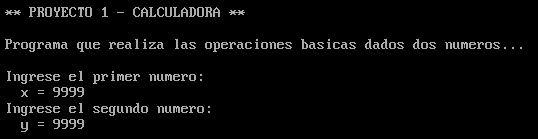
\includegraphics[width=0.95\textwidth]{img/01.png}
    \caption{Lectura de números}
    \end{figure}

    \subsubsection{printNumero}

    En este proceso, al imprimir el número se irán realizando divisiones para obtener el dígito más significativo al mismo tiempo que se hará uso de la variable $temp$ para ir guardando el residuo y repetir el proceso hasta obtener todos los dígitos, aquí se hace uso de la macro \textit{printDigito} para ir mostrando cada una de los dígitos. El primer número entre el cual se divide es $10000$ debido a que la mayor cantidad de cifras es de 5.

\begin{verbatim}
...
printNumero proc             ; procedimiento para imprimir el número

    mov bx,10000             ; BX = 10000
    xor dx,dx                ; DX = 0000h
    div bx                   ; DX:AX = AX / BX
    mov temp,dx              ; temp = DX

    printDigito al

    mov ax,temp              ; AX = temp

    mov bx,1000              ; BX = 1000
    xor dx,dx                ; DX = 0000h
    div bx                   ; DX:AX = AX / BX
    mov temp,dx              ; temp = DX

    printDigito al

    mov ax,temp              ; AX = temp

    mov bx,100               ; BX = 100
    xor dx,dx                ; DX = 0000h
    div bx                   ; DX:AX = AX / BX
    mov temp,dx              ; temp = DX

    printDigito al

    mov ax,temp              ; AX = temp

    mov bx,10                ; BX = 10
    xor dx,dx                ; DX = 0000h
    div bx                   ; DX:AX = AX / BX
    mov temp,dx              ; temp = DX

    printDigito al

    mov ax,temp              ; AX = temp

    printDigito al

    ret
endp printNumero
...
\end{verbatim}

    Dadas las condiciones del proyecto, este procedimiento debe ser adaptativo a números de 4 o 5 dígitos, por lo que en el código del procedimiento se incluye una comparación que nos permite avanzar en la ejecución de acuerdo al número de dígitos que conformen al número.

\begin{verbatim}
...
printNumero proc             ; procedimiento para imprimir el número
    cmp cl,5                 ; Compara CL con 5
    jb imprime4              ; Si CL < 5 entonces imprime solo 4 dígitos

    mov bx,10000             ; BX = 10000
    xor dx,dx                ; DX = 0000h
    div bx                   ; DX:AX = AX / BX
    mov temp,dx              ; temp = DX

    printDigito al

    mov ax,temp              ; AX = temp
imprime4:
    mov bx,1000              ; BX = 1000
    xor dx,dx                ; DX = 0000h
    div bx                   ; DX:AX = AX / BX
    mov temp,dx              ; temp = DX

    printDigito al

    mov ax,temp              ; AX = temp

    mov bx,100               ; BX = 100
    xor dx,dx                ; DX = 0000h
    div bx                   ; DX:AX = AX / BX
    mov temp,dx              ; temp = DX

    printDigito al

    mov ax,temp              ; AX = temp

    mov bx,10                ; BX = 10
    xor dx,dx                ; DX = 0000h
    div bx                   ; DX:AX = AX / BX
    mov temp,dx              ; temp = DX

    printDigito al

    mov ax,temp              ; AX = temp

    printDigito al

    ret
endp printNumero
...
\end{verbatim}

    NOTA: Es importante mencionar que esta implementación llenará de 0's a la izquierda para completar las cuatro o cinco cifras según sea el caso.

    \subsection{Suma}
    La suma requiere de la impresión de 5 cifras, pues al ingresar máximo 4 dígitos en cada número y suponiendo que ingresan el número mayor dos veces, i.e. $9999$, el resultado máximo obtenible es $19998$.

    Una vez sabido esto, el proceso para realizar la suma es muy simple:

    \begin{enumerate}
        \item Realizar la suma de $num1$ mas $num2$.
        \item Guardar el resultado obtenido en la variable $suma$.
        \item Imprimir un mensaje para el usuario.
        \item Indicar el número de dígitos.
        \item Imprimir el resultado.
    \end{enumerate}

    En lenguaje ensamblador queda de la siguiente manera:

    \begin{verbatim}
...
suma:
    mov ax,num1        ; AX = num1
    add ax,num2        ; AX = AX + num2
    mov sum,ax         ; sum = AX

    mov ah,09h         ; Prepara registro ah para imprimir un mensaje en pantalla
    lea dx,msjSuma     ; Imprime mensaje de suma
    int 21h            ; Interrupcion 21h para controlar funciones del S.O.

    mov ax,sum         ; AX = sum

    mov cl,5           ; Indica el número de dígitos
    call printNumero   ; Imprime el número
...
    \end{verbatim}

    \begin{figure}[H]
    \centering
    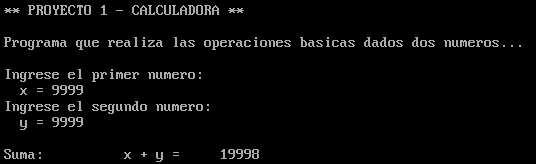
\includegraphics[width=0.8\textwidth]{img/02.png}
    \caption{Imprime suma}
    \end{figure}

    \subsection{Resta}

    A diferencia de la suma, para las siguientes operaciones es necesario de utilizar los registros $AX$ y $BX$ para guardar el valor de $num1$ y $num2$ respectivamente.

    Para el caso particular de la resta, esto es necesario para realizar las comparaciones necesarias para verificar cuál de los dos números es mayor y de esta manera siempre obtener como resultado de la operación un número entero sin signo.

    Dependiendo de cuál de los dos números se elija como el mayor se imprimirá (o no) el caracter `-', con valor hexadecimal $2Dh$.

    Por ejemplo:

    Si $num1 = 12$ y $num2 = 5$ el programa realizará la operación $12 - 5$ y el resultado será $7$, por otro lado si $num1 = 5$ y $num2 = 12$ el programa también realizará la operación $12 - 5$ pero mostrará en pantalla $-7$.

    Para esto nos auxiliaremos de la variable $nega$ que hará la emulación de una varible booleana que podrá contener un 0 o un 1 y nos servirá para indicar al programa si imprime o no el signo menos.

    \begin{enumerate}
        \item Compara cuál de los dos números es mayor.
        \item Realizar la resta del mayor menos el menor.
        \item Guardar el resultado obtenido en la variable $res$.
        \item Imprimir un mensaje para el usuario.
        \item Si $nega=0$ imprime un `$-$'.
        \item Indicar el número de dígitos.
        \item Imprimir el resultado.
    \end{enumerate}

    Para saber la cantidad necesaria de digitos para la impresión del resultado de la resta partimos de la suposición de restar el menor número posible al mayor número posible, i.e. $9999$ menos $0$.

    Como se puede observar, el resultado máximo es un número de cuatro cifras, por lo que será necesario indicarlo al procedimiento de impresión, es tan simple como asignar el valor $4$ al registro $CL$.

\begin{verbatim}
...
resta:
    mov ax,num1        ; AX = num1
    mov bx,num2        ; BX = num2
    cmp ax,bx          ; Compara AX con BX
    jb menor           ; Si el primer numero es menor que el 
                       ; segundo entonces brinca a etiqueta 'menor'
    sub ax,num2        ; Si el primer numero es mayor que el segundo 
                       ; realiza la resta directamente, AX = AX - num2
    mov res,ax         ; res = AX
    jmp flujo4         ; Brinca al flujo4 para imprimir el resultado

menor:
    sub bx,num1        ; Como el primero es menor entonces resta 
                       ; el primer numero al segundo, BX = BX - num1
    mov res,bx         ; res = BX
    add nega,1         ; nega = nega + 1, esta operacion sirve para 
                       ; comparar si el resultado debe ser negativo o no

flujo4:
    mov ah,09h         ; Prepara registro ah para imprimir un mensaje
    lea dx, msjResta   ; Imprime el mensaje de Resta
    int 21h            ; Interrupcion 21h para controlar funciones del S.O.

    mov cl,nega        ; CL = nega
    cmp cl,1           ; Compara CL con 1
    jne positivo       ; Si CL != 1 quiere decir que el numero es positivo 
                       ; y por lo tanto sigue el flujo normal
    mov ah,02h         ; AH = 02H, prepara AH para imprimir un caracter
    mov dl,2Dh         ; DL = 2Dh, 2Dh es el codigo equivalente 
                       ; al simbolo del signo negativo
    int 21h            ; Interrupcion 21h para controlar funciones del S.O.
    sub nega,1         ; nega = nega - 1, limpia la variable 'nega'

positivo:
    cmp cl,1           ; Compara CL con 1
    je flujo5          ; Si CL == 1, si es negativo entonces continua 
                       ; con el flujo normal
    mov ah,02h         ; AH = 02H, prepara AH para imprimir un caracter
    mov dl,20h         ; DL = 20h, imprime un espacio en blanco
    int 21h            ; Interrupcion 21h para controlar funciones del S.O.
flujo5:
    mov ax,res         ; AX = res

    mov cl,4
    call printNumero   ; Imprime el número 
...
\end{verbatim}

    \begin{figure}[H]
    \centering
    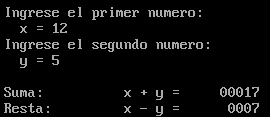
\includegraphics[width=0.8\textwidth]{img/03.png}
    \caption{Imprime resta positiva}
    \end{figure}

    \begin{figure}[H]
    \centering
    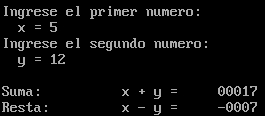
\includegraphics[width=0.8\textwidth]{img/04.png}
    \caption{Imprime resta negativa}
    \end{figure}

    NOTA: Es importante tener en cuenta que el valor que almacena la variable $res$ es un número entero sin signo, por lo que esta solución es solo estética y para dar una buena presentación.

    \subsection{Multiplicación}
    \subsection{División}
    \subsection{Menu}
    \newpage
    \section{Diagramas de Flujo.}
    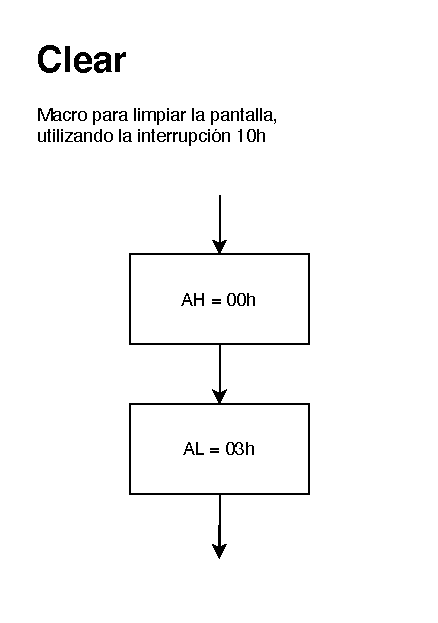
\includegraphics[width=0.48\textwidth]{img/diagramas/p01-Clear}
    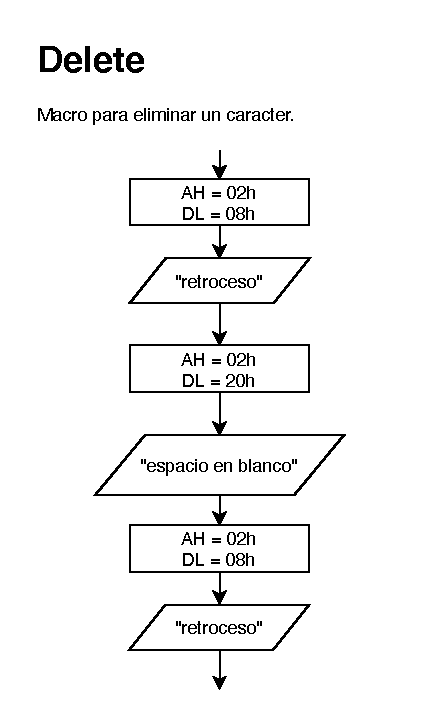
\includegraphics[width=0.47\textwidth]{img/diagramas/p01-Delete}

    \begin{center}
    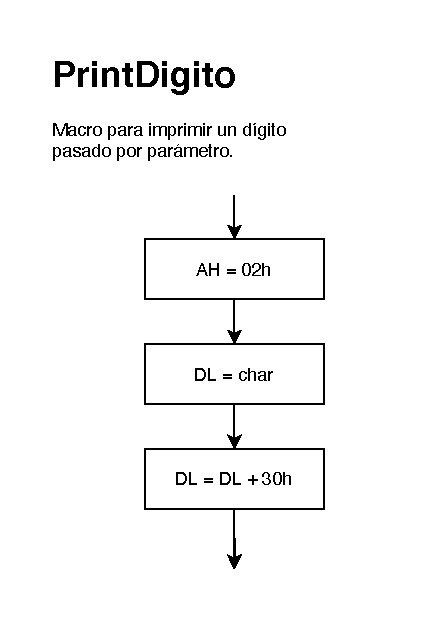
\includegraphics[width=0.5\textwidth]{img/diagramas/p01-PrintDigito}
    \end{center}

    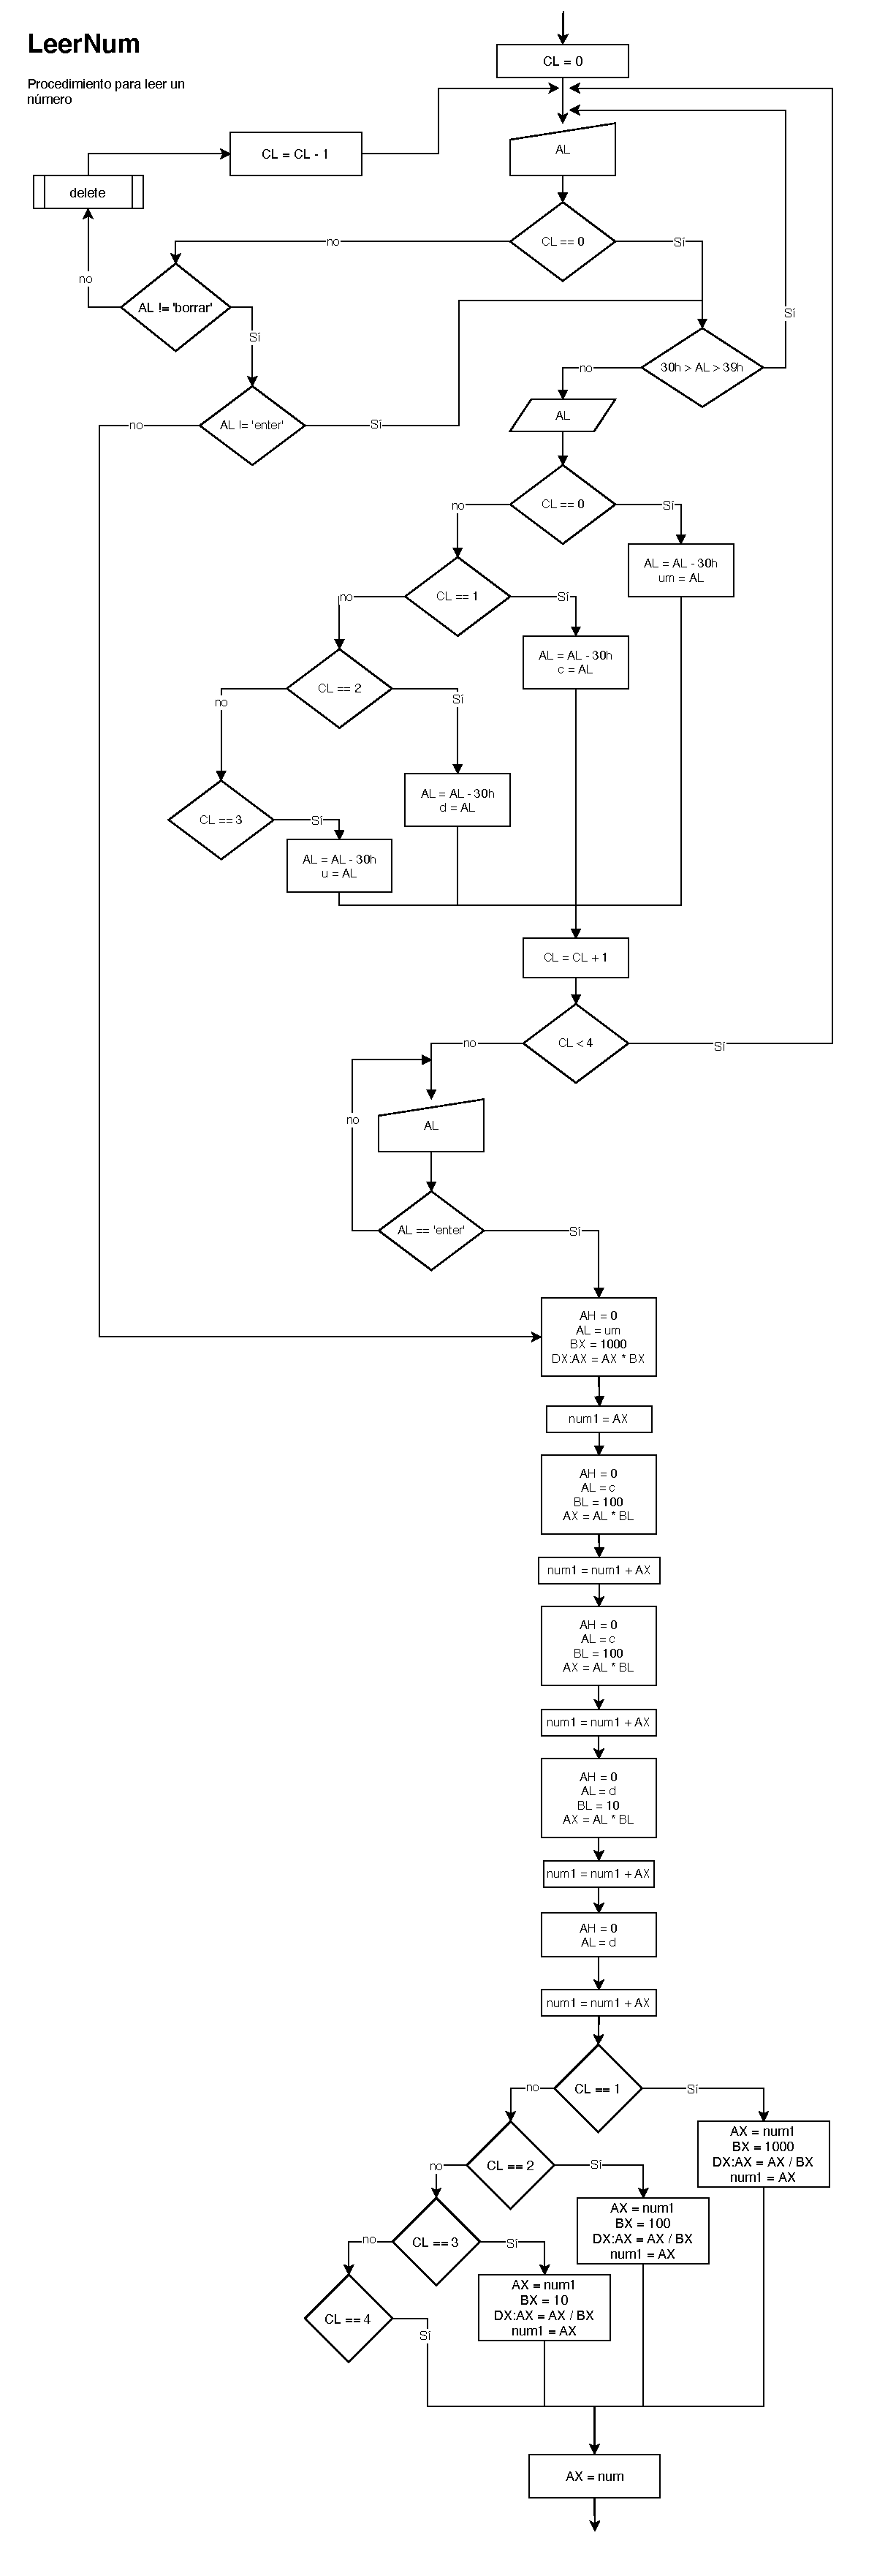
\includepdf[fitpaper=true]{img/diagramas/p01-LeerNum}
    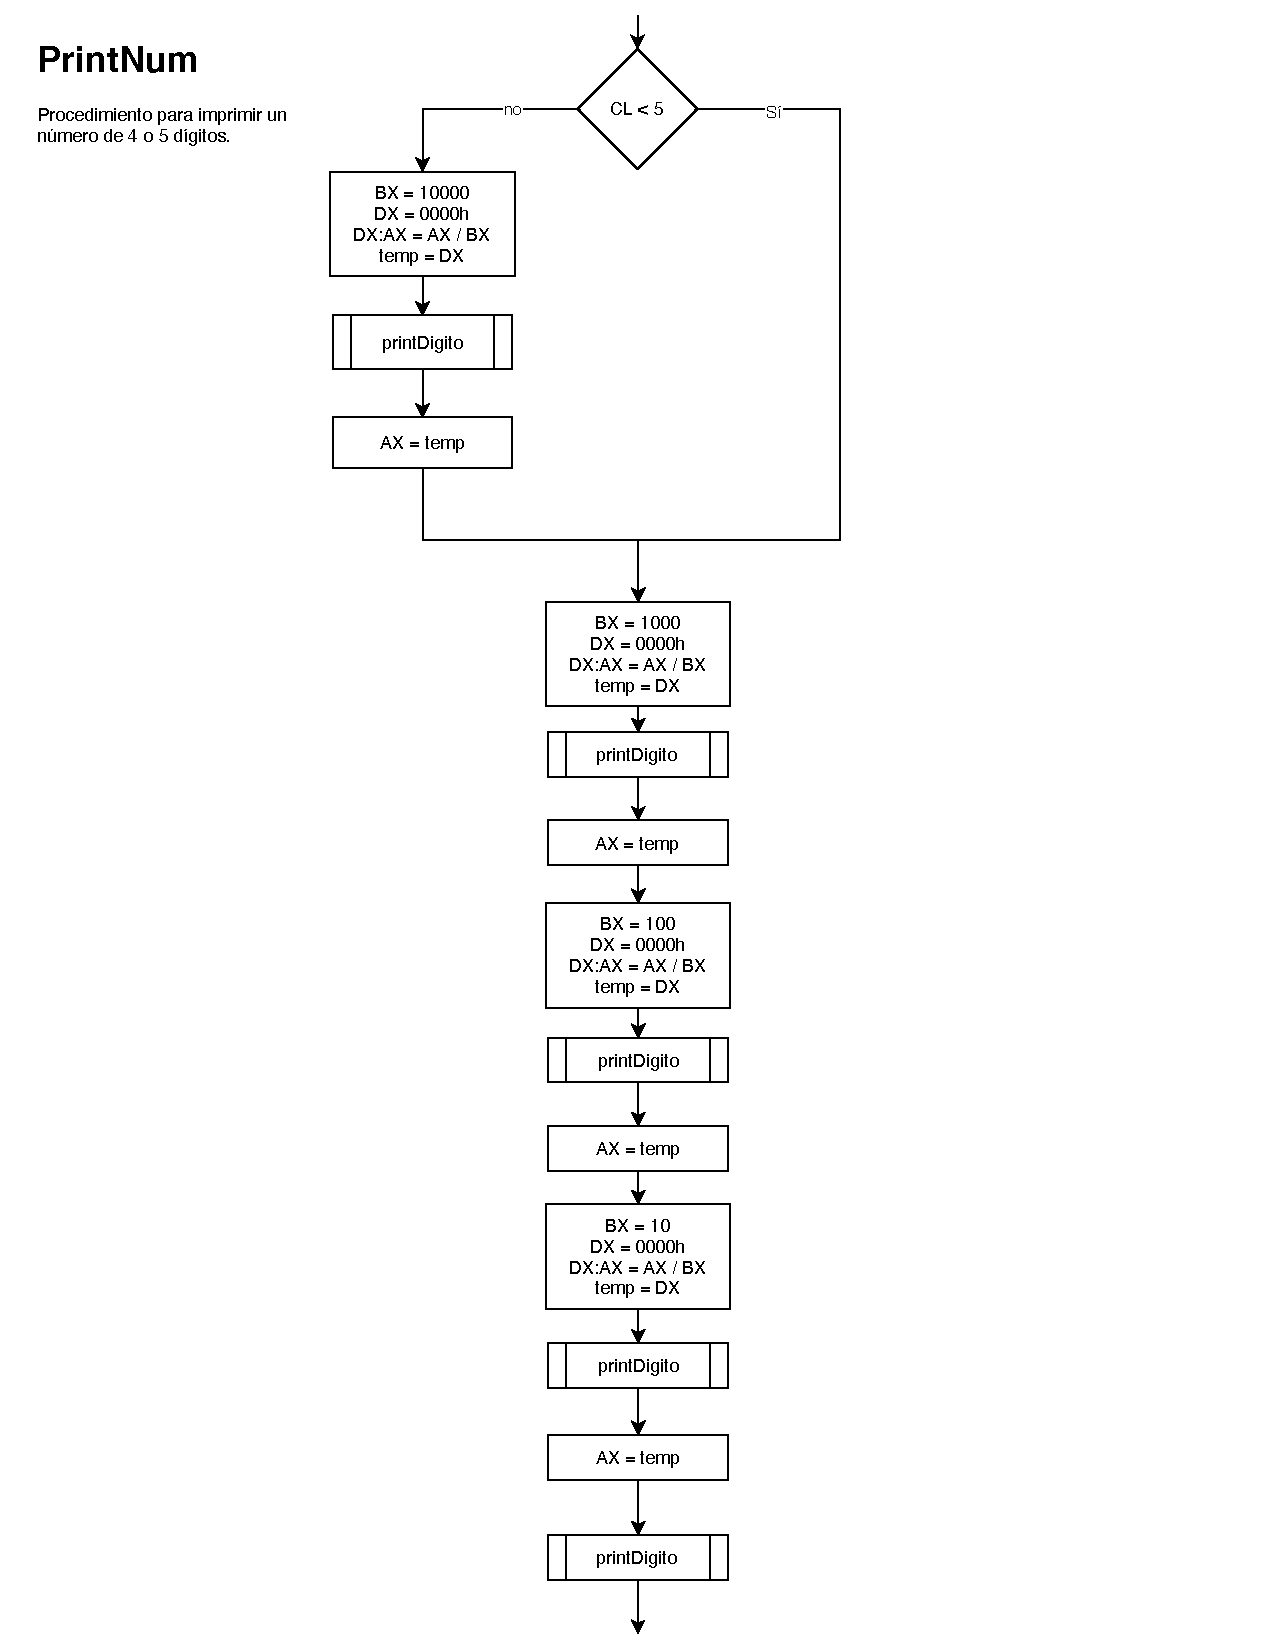
\includepdf[fitpaper=true]{img/diagramas/p01-PrintNum}
    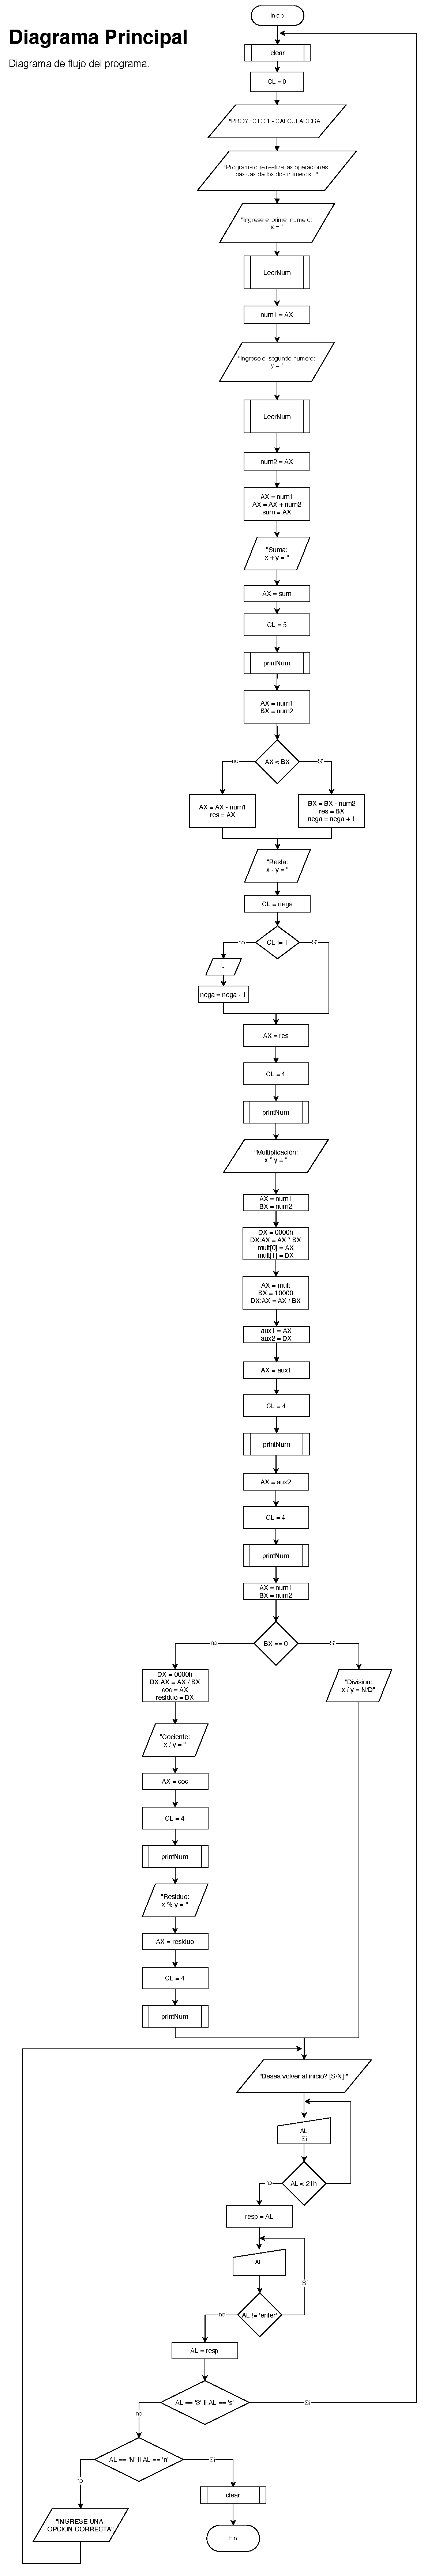
\includepdf[fitpaper=true]{img/diagramas/p01-DiagramaFlujo}

    \section{Pruebas de Escritorio}

    La pruebas de escritorio se realizarán utilizando dos números: $4321$ y $123$, se llevarán siguiendo las operaciones mostradas en los diagramas de flujo de \textit{leerNum} y \textit{Diagrama Principal}.

    La prueba de escritorio para imprimir un número solo se realizará para el residuo de la división debido a que todas las impresiones siguen la misma metodología.

    \subsection{leerNum}

    \begin{center}
    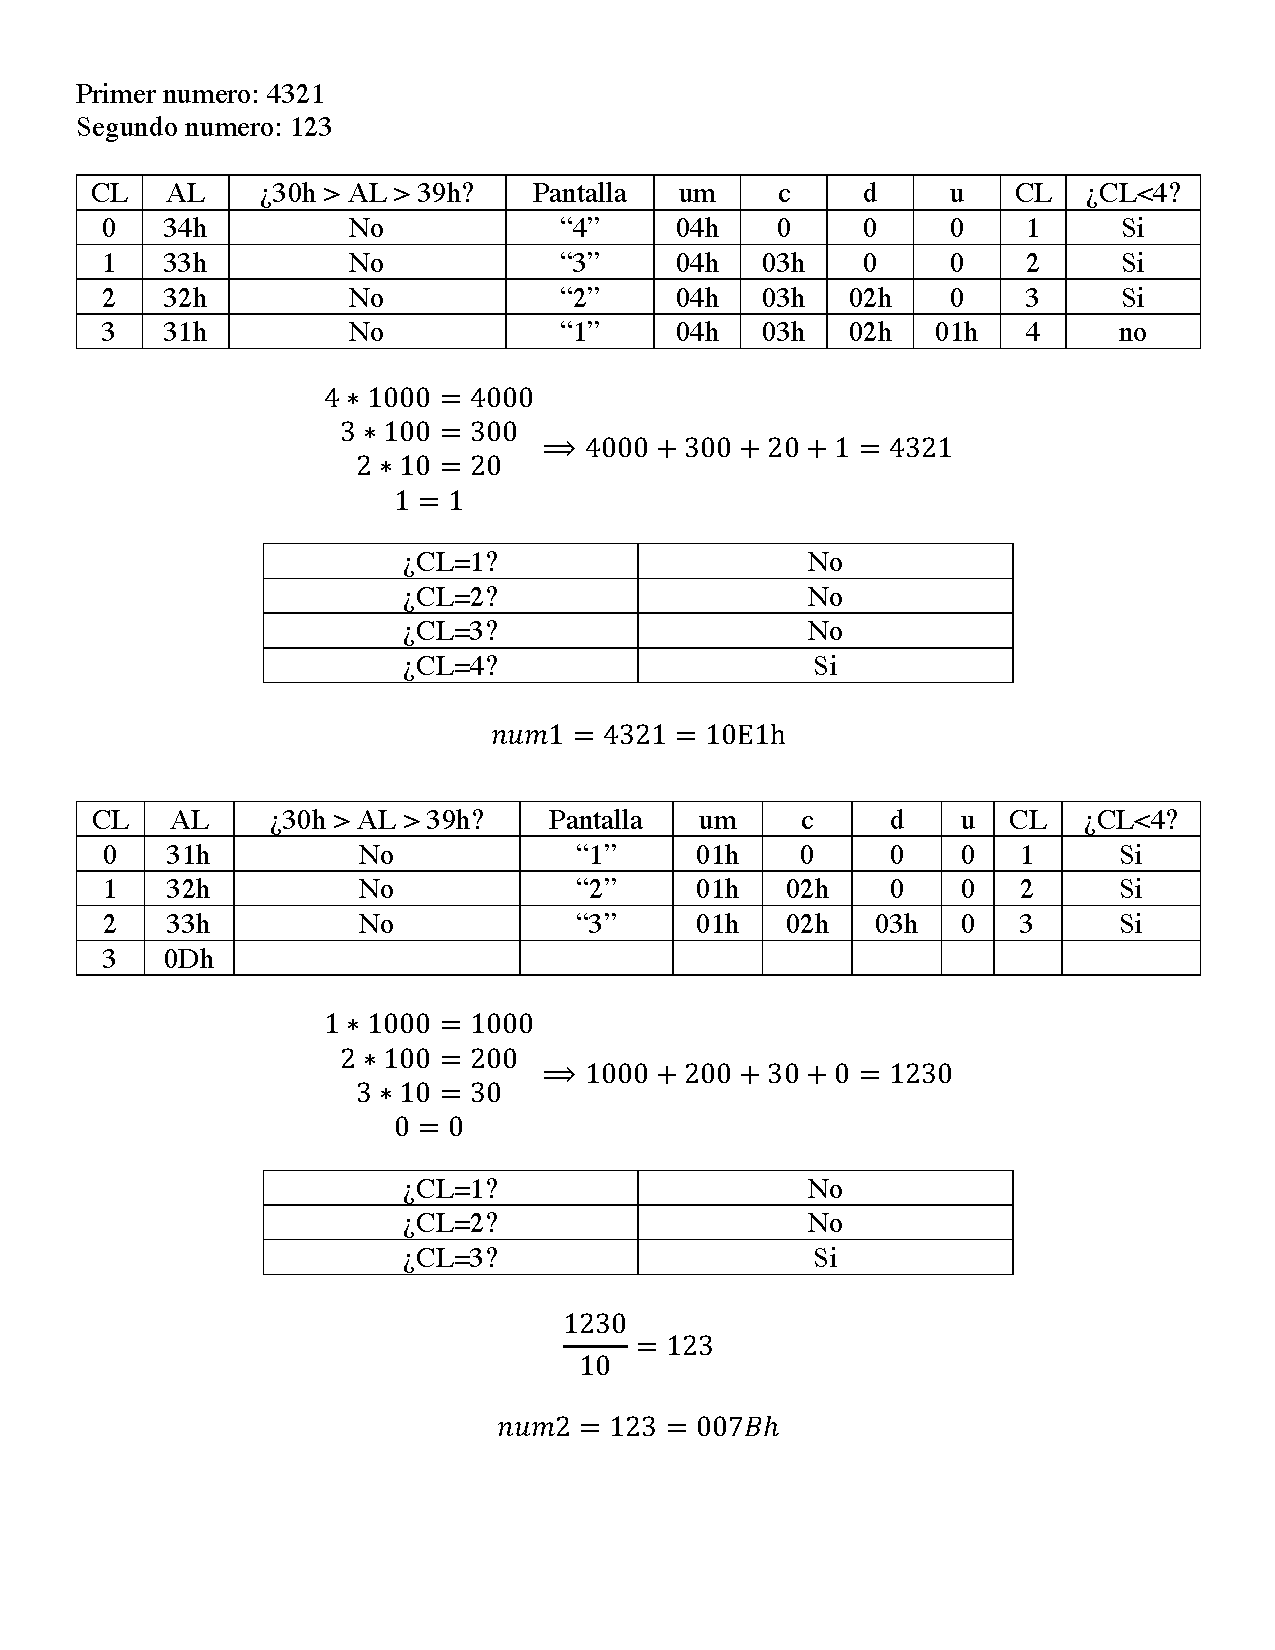
\includegraphics[width=0.95\textwidth]{img/Primer numero.pdf}
    \end{center}

    \subsection{Diagrama Principal}

    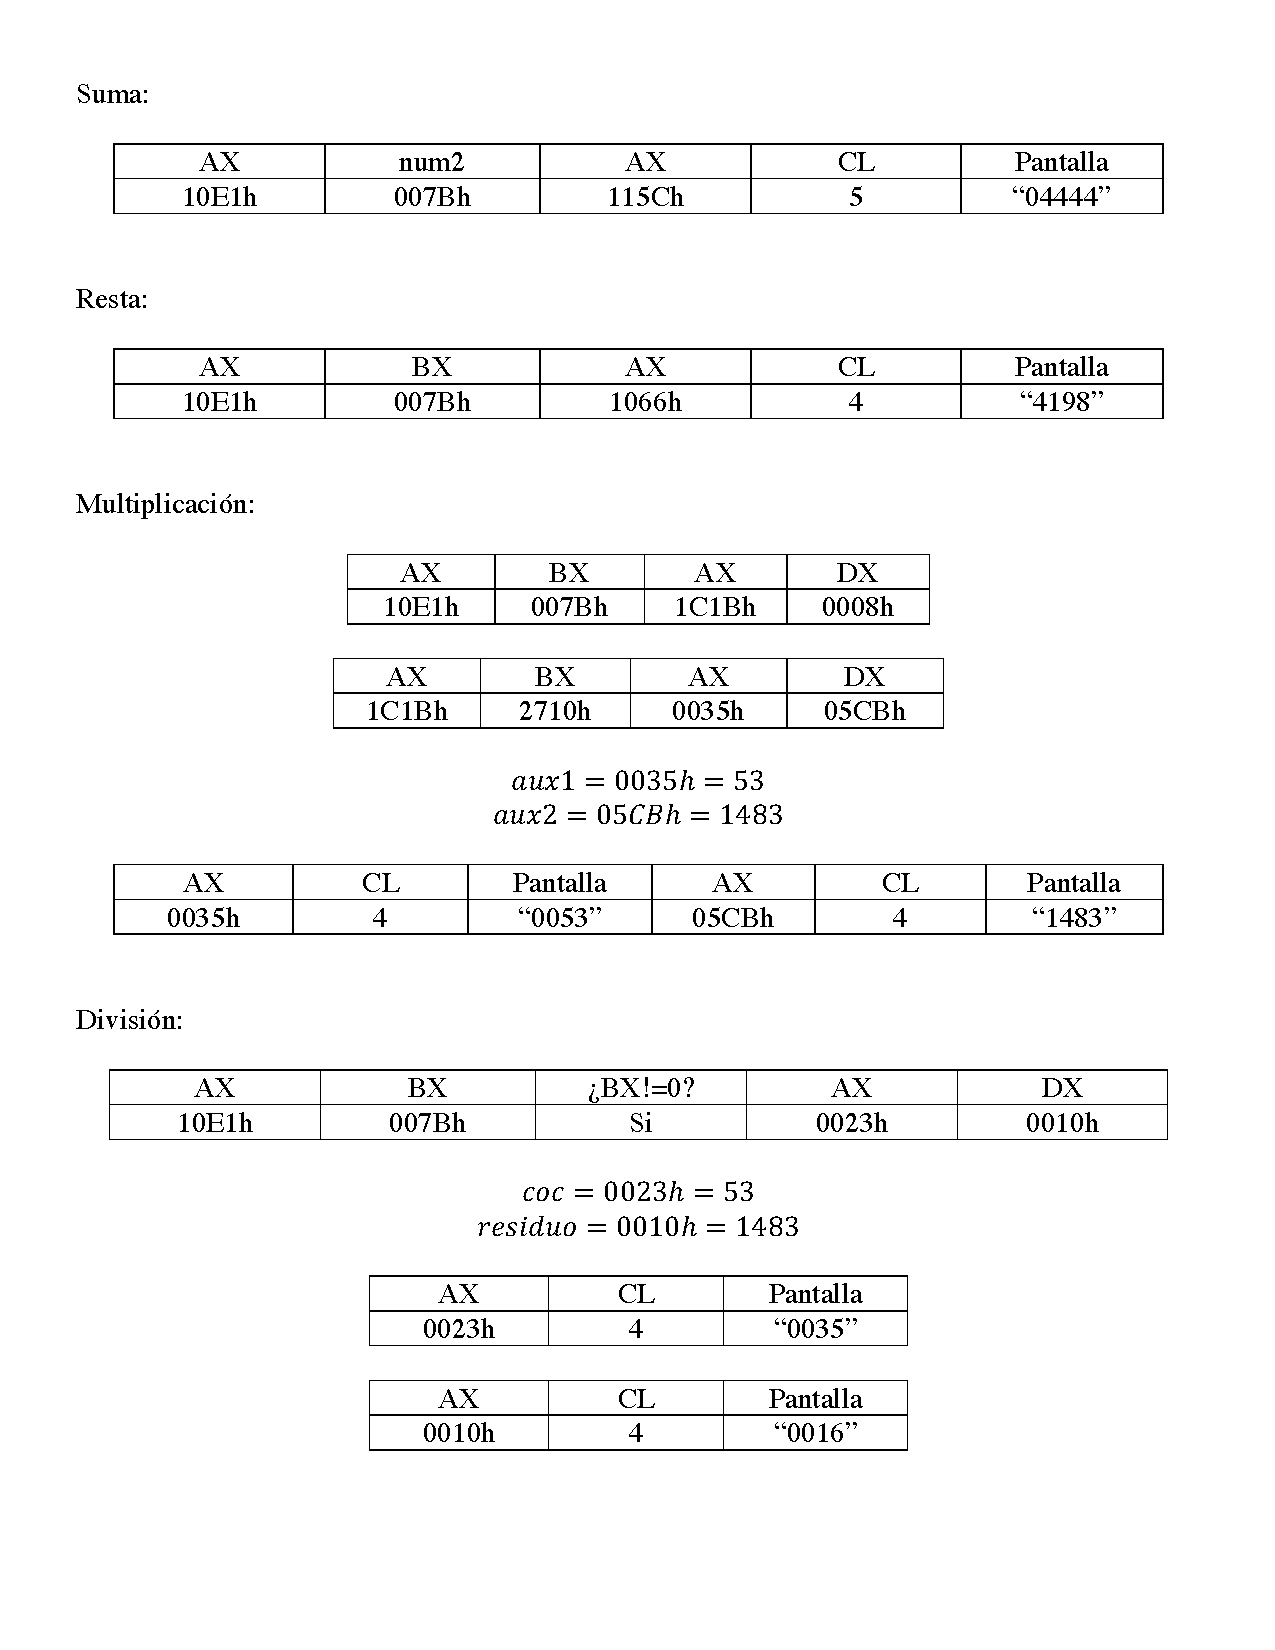
\includegraphics[width=1\textwidth]{img/Suma.pdf}

    \subsection{Impresión}

    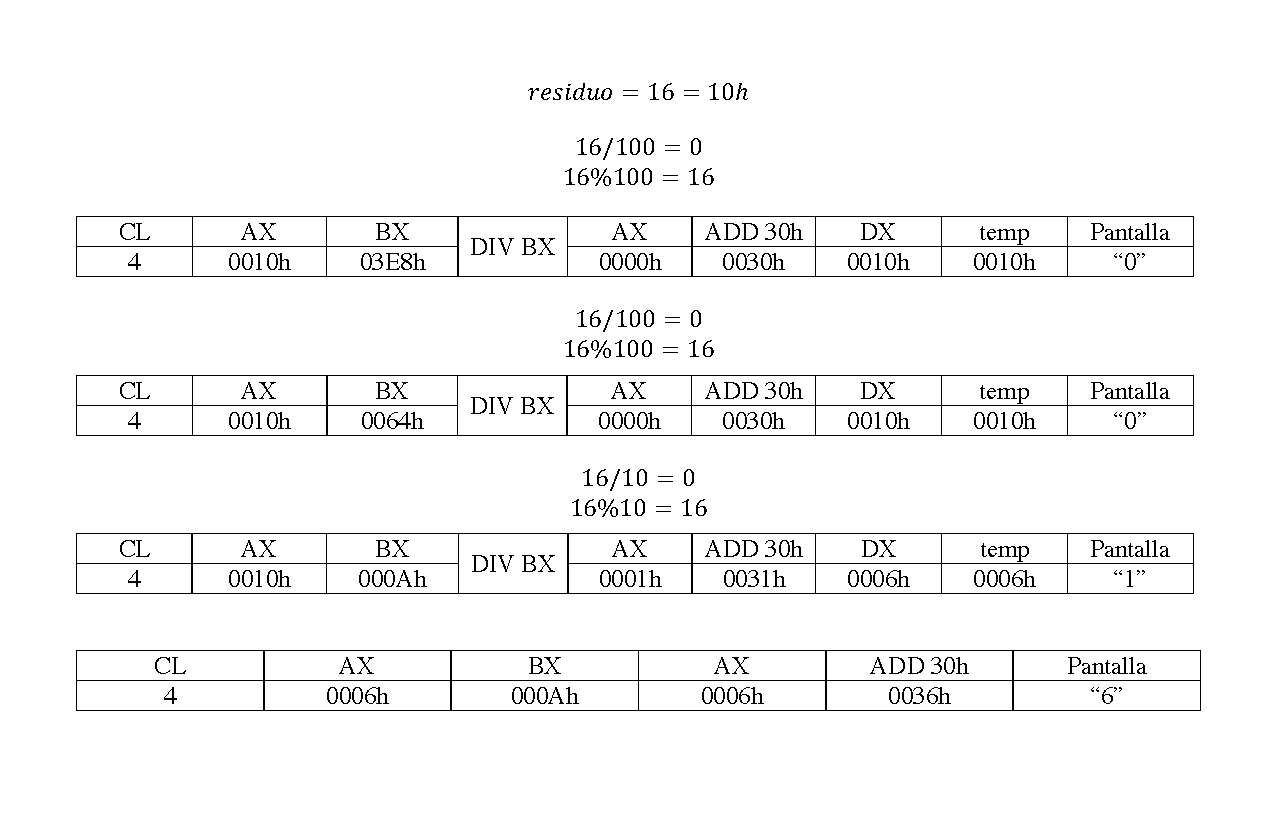
\includegraphics[width=1\textwidth]{img/residuo.pdf}
    
    \section{Conclusión}

    Para lograr la correcta implementación de la solución del proyecto, fue necesario el uso constante del \textit{turbo debugger}, pues este ayudó al mostrarnos el comportamiento de los registros en cada una de las líneas de ejecución y de esta manera ir comprendiendo la naturaleza de las operaciones del ensamblador.

    La ayuda del profesor, tanto en horario de clase como fuera del mismo propició una resolución temprana del problema, y a su vez una optimización del código en cuanto a la extensión y funcionalidades del mismo.

    Lo más difícil del proyecto fue la parte de lectura e impresión de números, pues una vez que se logró implementarse, el resto de la solución no presentó problemas a la hora de programar.

    Otro elemento importante al momento de realizar este proyecto fue el uso de etiquetas y saltos condicionales, pues es parte fundamental de la solución del problema, es por esto que considero a este trabajo un pilar firme para nuestro aprendizaje sobre las operaciones básicas y condicionales en lenguaje ensamblador.

    Para finalizar también cabe mencionar que gracias a las clases más recientes de la asignatura de Estructura y Programación de Computadoras fue posible implementar el uso de macroinstrucciones y procedimientos en la estructura del código presentado.

\end{document}





